\documentclass[tikz,border=10pt]{standalone}
\usepackage{tikz}
\usetikzlibrary{shapes,arrows,positioning}
\usepackage{amsmath}

\definecolor{fepblue}{RGB}{41,128,185}
\definecolor{crrgreen}{RGB}{39,174,96}
\definecolor{goalred}{RGB}{192,57,43}
\definecolor{matchpurple}{RGB}{142,68,173}

\begin{document}
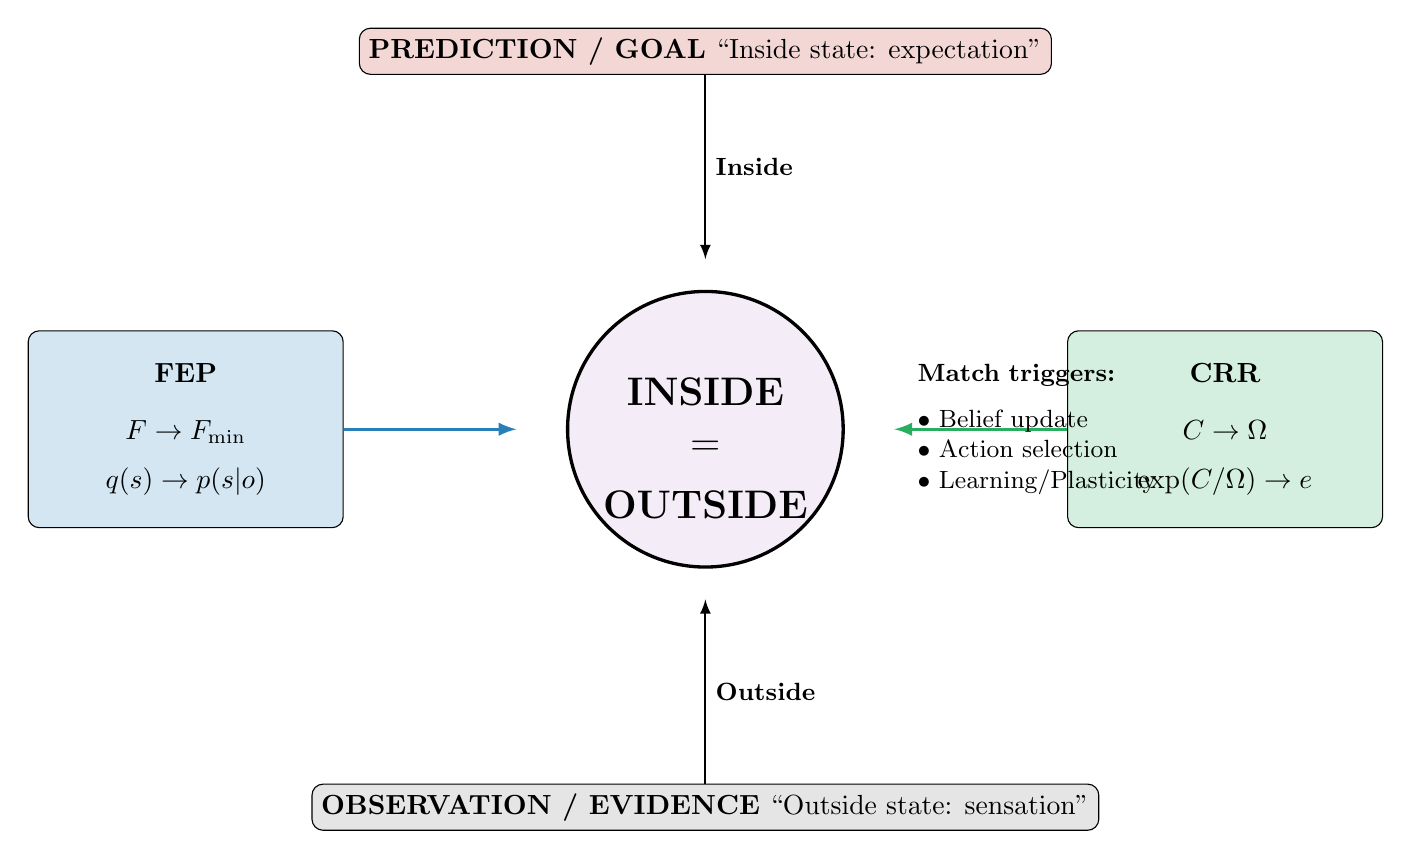
\begin{tikzpicture}[scale=1.2]
% Central diagram
\node[draw, very thick, circle, minimum size=35mm, fill=matchpurple!10] (center) at (0,0) {};
\node[font=\Large\bfseries] at (0,0.4) {INSIDE};
\node[font=\Large\bfseries] at (0,-0.2) {$=$};
\node[font=\Large\bfseries] at (0,-0.8) {OUTSIDE};

% FEP side
\node[draw, rounded corners, fill=fepblue!20, minimum width=40mm, minimum height=25mm, align=center] (fep) at (-5.5,0) {
\textbf{FEP}\\[3mm]
$F \to F_{\min}$\\[2mm]
$q(s) \to p(s|o)$
};

% CRR side
\node[draw, rounded corners, fill=crrgreen!20, minimum width=40mm, minimum height=25mm, align=center] (crr) at (5.5,0) {
\textbf{CRR}\\[3mm]
$C \to \Omega$\\[2mm]
$\exp(C/\Omega) \to e$
};

% Arrows
\draw[-latex, very thick, fepblue] (fep) -- (-2,0);
\draw[-latex, very thick, crrgreen] (crr) -- (2,0);

% Top: Prediction
\node[draw, rounded corners, fill=goalred!20, minimum width=60mm] (pred) at (0,4) {
\textbf{PREDICTION / GOAL}\\[1mm]
``Inside state: expectation''
};

% Bottom: Observation
\node[draw, rounded corners, fill=gray!20, minimum width=60mm] (obs) at (0,-4) {
\textbf{OBSERVATION / EVIDENCE}\\[1mm]
``Outside state: sensation''
};

% Vertical arrows
\draw[-latex, thick] (pred) -- (0,1.8) node[midway, right, font=\small\bfseries] {Inside};
\draw[-latex, thick] (obs) -- (0,-1.8) node[midway, right, font=\small\bfseries] {Outside};

% Match annotation
\node[right=8mm of center, font=\small, text width=35mm, align=left] {
\textbf{Match triggers:}\\[2mm]
$\bullet$ Belief update\\
$\bullet$ Action selection\\
$\bullet$ Learning/Plasticity
};
\end{tikzpicture}
\end{document}
